\section{Appendix to Section \ref{s:assertions} -- Assertions}
\label{appendix:assertions}

Figure \ref{fig:ProtectedFrom} illustrates ``protected from'' and ``protected''. % protection from other objects. 
In the first row  we  highlight in yellow  the objects protected from other objects. Thus, all objects except $o_6$ are protected from $o_5$ (left pane);\ all objects expect $o_8$ are protected from $o_7$ (middle pane);\ and all objects except $o_3$, $o_6$, $o_7$, and $o_8$ are protected from $o_2$ (right pane). 
Note  that $o_6$ is not protected from $o_2$, because  $o_5$ is reachable from $o_2$, is external, and has direct access to $o_6$.

In the third row of   Figure \ref{fig:Protected} we show three states: 
 $\sigma_1$ has  top frame $\phi_1$, which has  one variable, \prg{this}, pointing to $o_1$, while 
 $\sigma_2$ has  top frame $\phi_2$; it has two  variables,   \prg{this} and \prg{x} pointing to $o_3$ and  $o_7$, and 
 $\sigma_3$ has  top frame $\phi_3$; it has two  variables,  \prg{this} and \prg{x}, pointing to $o_7$ and $o_3$.  
% 
%The locally reachable objects in $\sigma_1$ were highlighted in the middle pane of Fig \ref{fig:LReachable}; 
%the locally reachable objects from $\sigma_2$  are the same as those from $\sigma_3$, and  were  highlighted in the right pane of that
%Fig. 
%In Fig.  \ref{gig:Protected} 
We also   highlight the protected objects with a yellow halo.
 Note that $o_3$ is protected in $\sigma_2$, but is not protected in $\sigma_3$. This is so, because $\interpret {\sigma_3} {\prg{this}}$  is external, and  $o_3$ is an argument to the call. As a result, during the call, $o_7$ may obtain direct access to $o_3$. 
 
\begin{figure}[tbh]
\begin{tabular}{|c|c|c|}
\hline  
\resizebox{4.5cm}{!}{
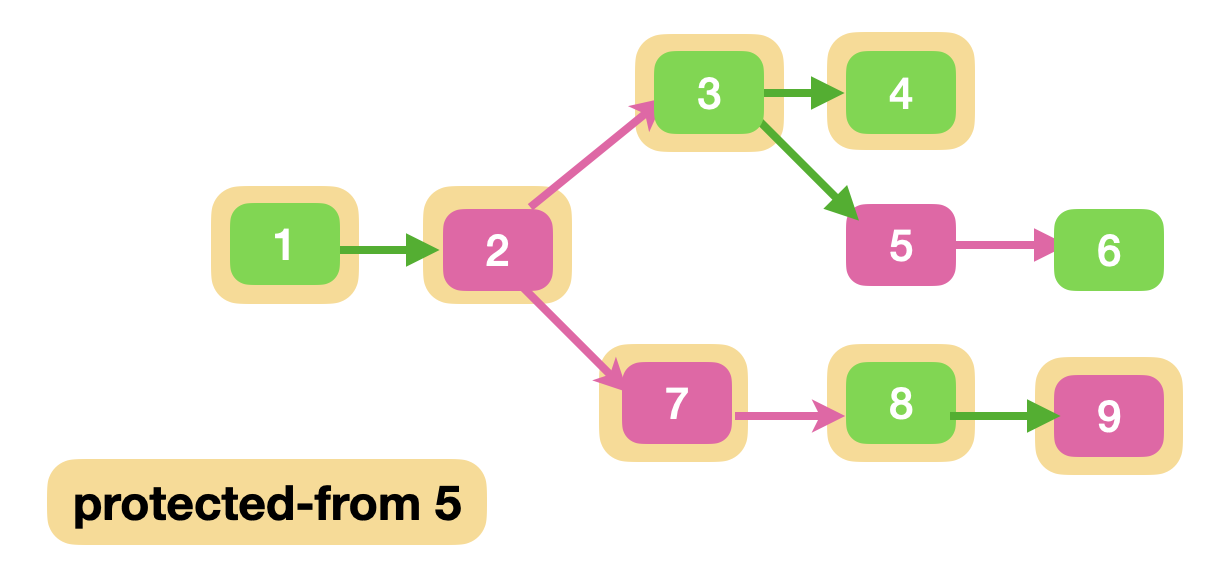
\includegraphics[width=\linewidth]{diagrams/prfA.png}
} 
&
\resizebox{4.5cm}{!}{
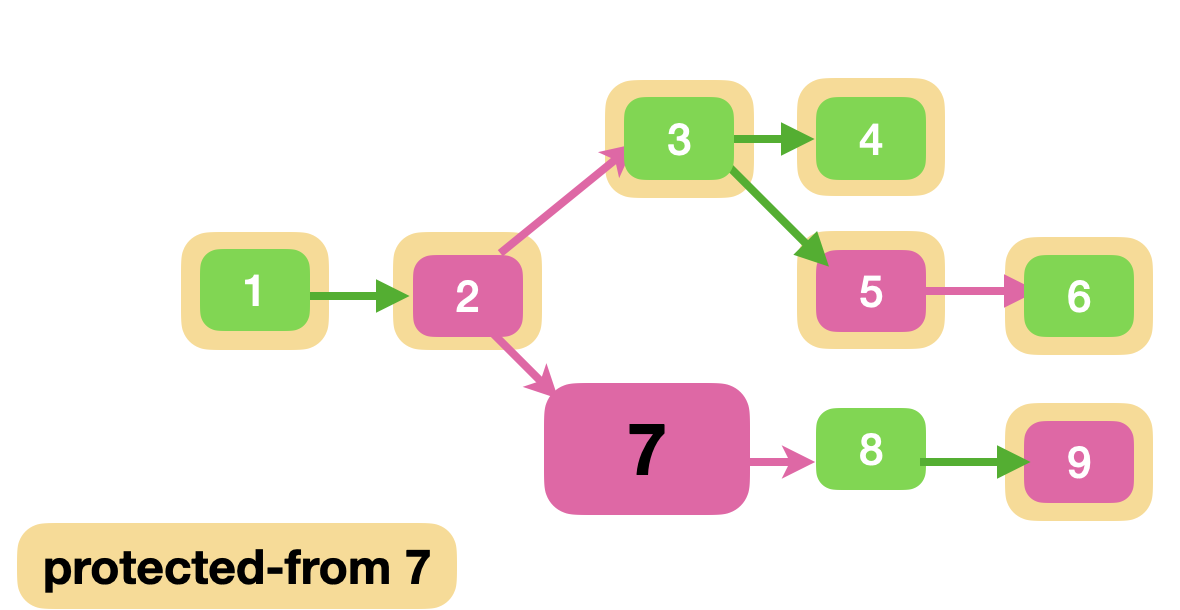
\includegraphics[width=\linewidth]{diagrams/prfB.png}
} 
&
\resizebox{4.5cm}{!}{
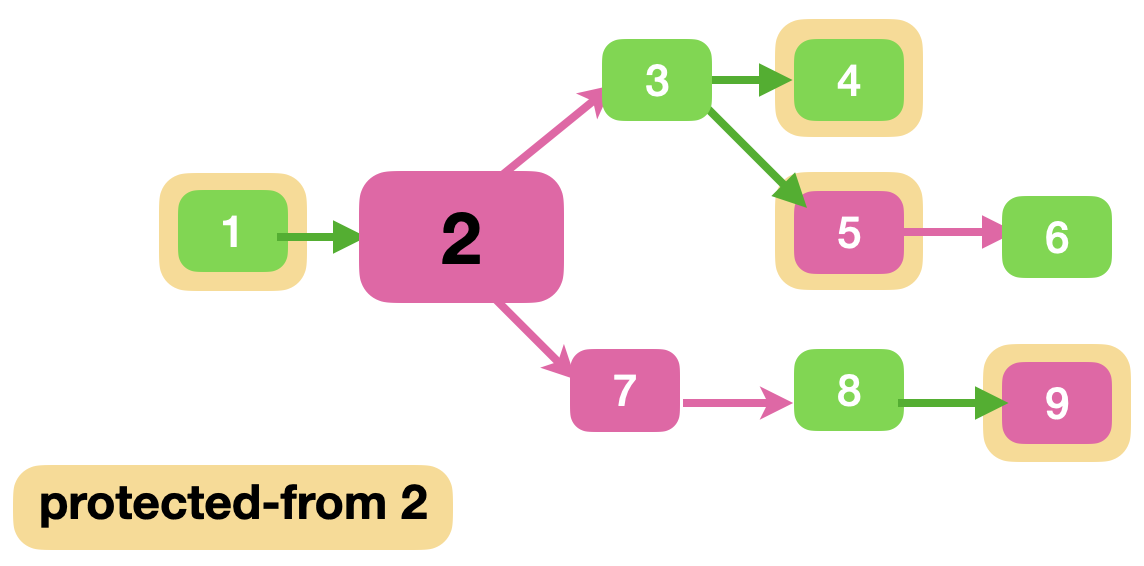
\includegraphics[width=\linewidth]{diagrams/prfC.png}
} 
\\
\hline
protected from $o_5$
&
protected from $o_7$
&
protected from $o_2$
\\
\hline  \hline
\resizebox{4.5cm}{!}{
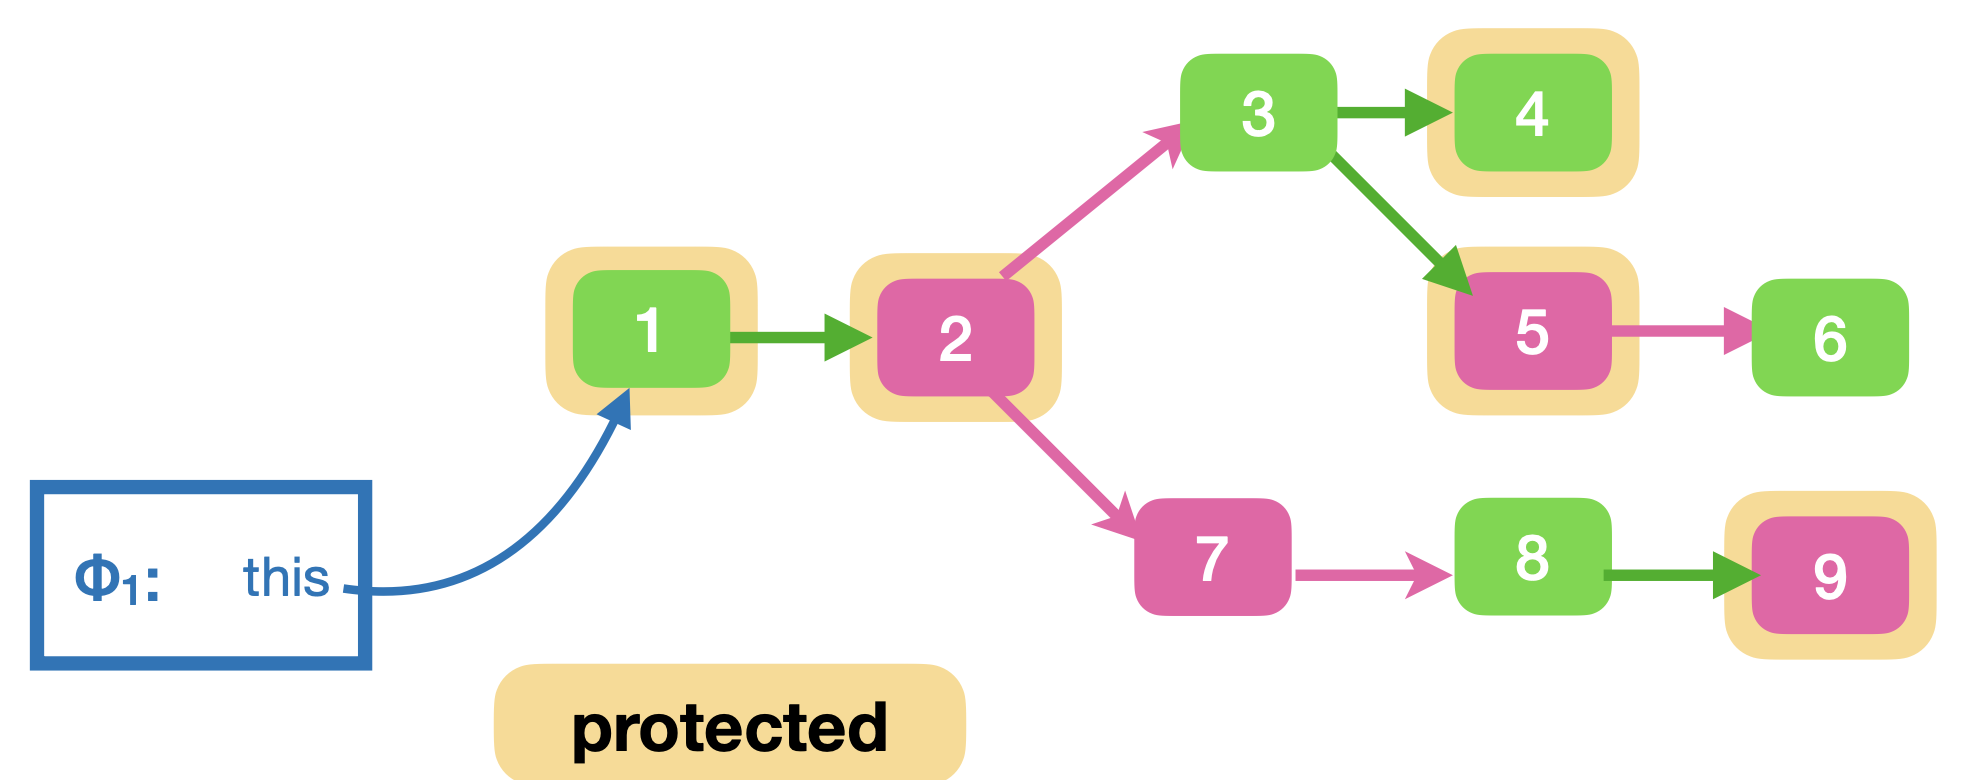
\includegraphics[width=\linewidth]{diagrams/prtFirst.png}
} 
&
\resizebox{4.5cm}{!}{
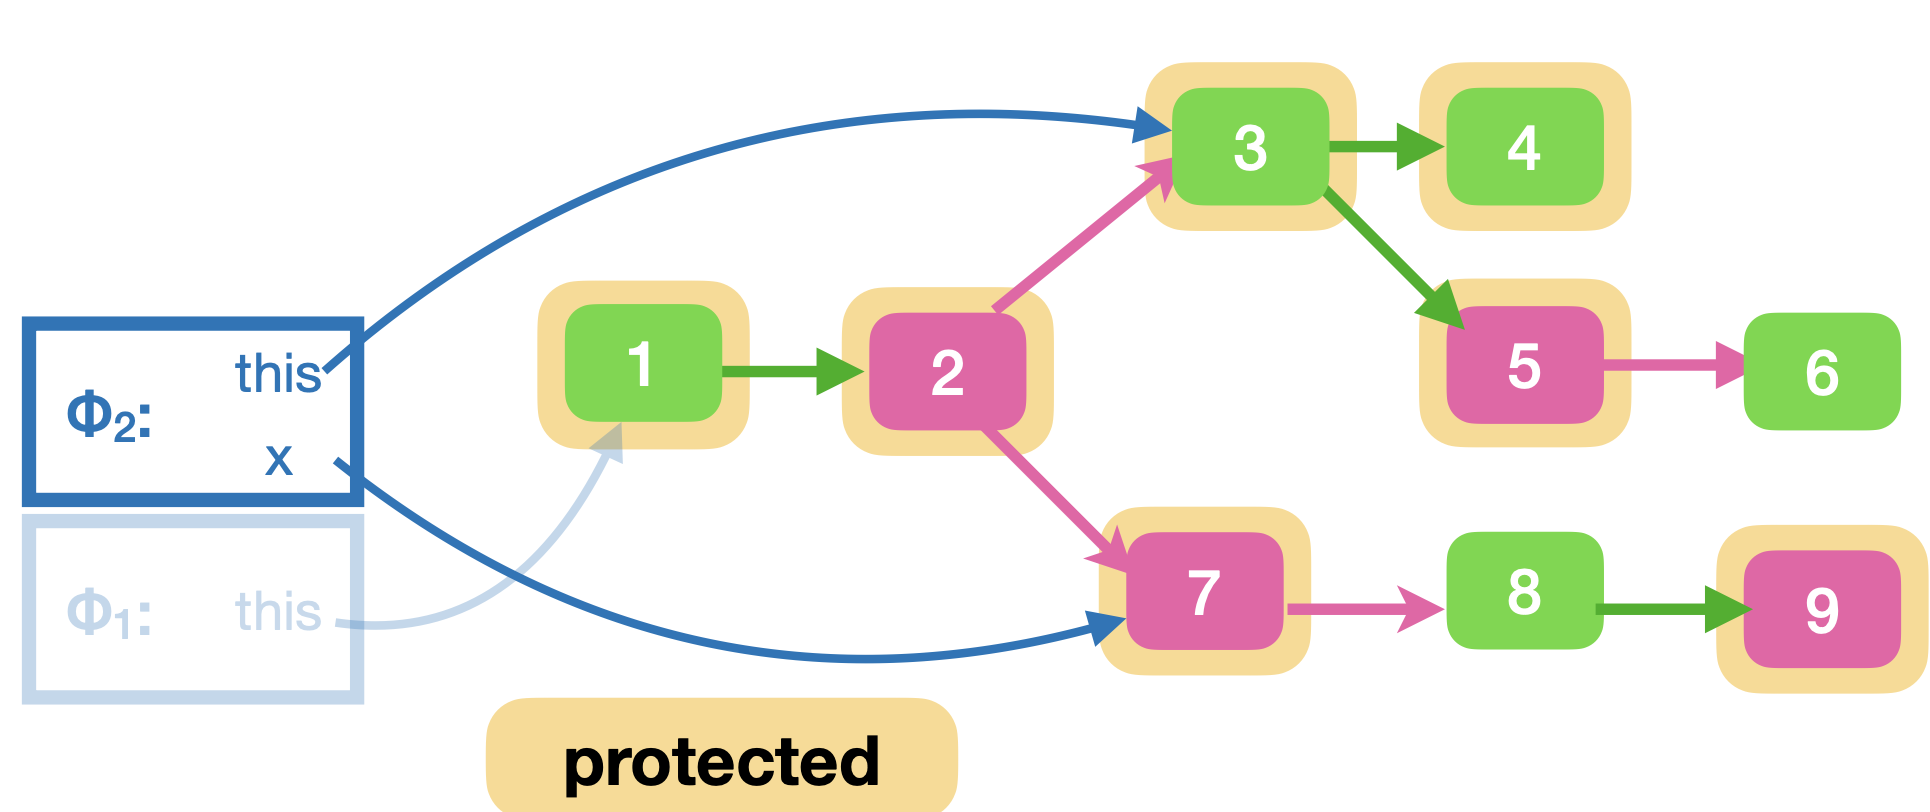
\includegraphics[width=\linewidth]{diagrams/prtSecond.png}
} 
&
\resizebox{4.5cm}{!}{
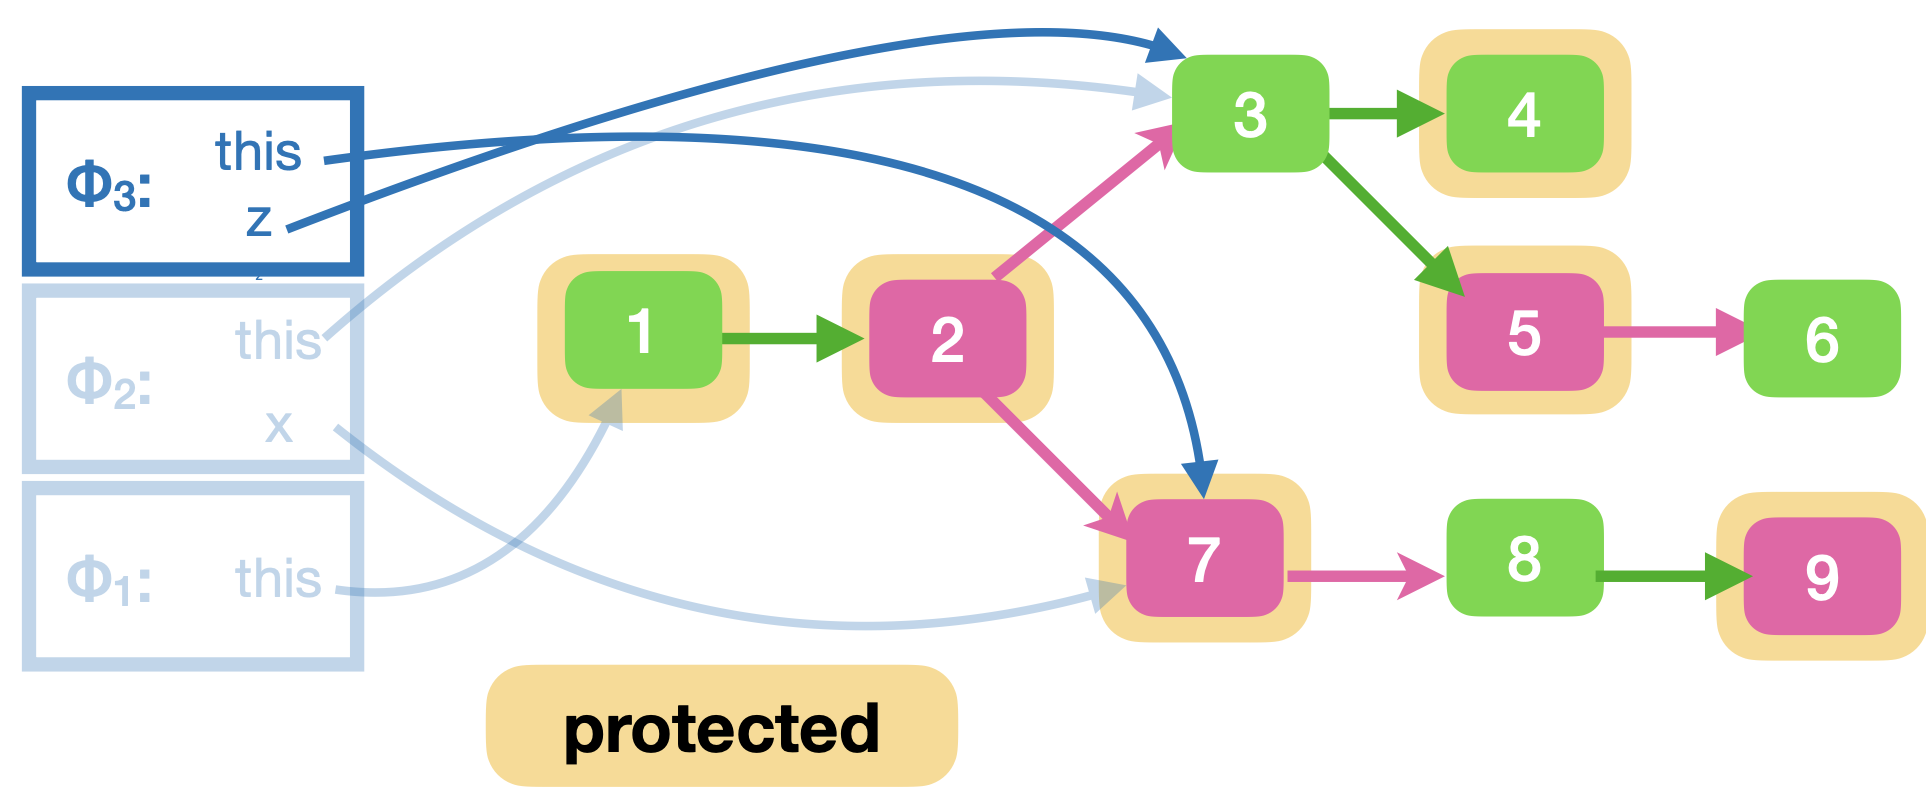
\includegraphics[width=\linewidth]{diagrams/prtLast.png}
} 
\\
\hline
protected in $\sigma_1$ & % with top frame $\phi_1$ &
protected   in $\sigma_2$ & % with top frame $\phi_2$ &
protected  in $\sigma_3$  % with top frame $\phi_2$ &
\\
\hline \hline
\end{tabular}
   \caption{ Protection. Pink objects are external, and green objects are internal.}
   \label{fig:ProtectedFrom}
    \label{fig:Protected}
 \end{figure}


\sdN{In order to prove \ref{lemma:addr:expr} from the next appendix, we first formulate and prove the following auxiliary lemma, which allows us to replace any variable $x$ in an extended expression $\re$, by its interpretation

\begin{lemma}
\label{aux:lemma:vars:eval}
For all extended expressions $\re$,  addresses $\alpha$ and  variables $x$, so that $x \in dom(\sigma):$

\begin{itemize}
\item
$\eval{M}{\sigma}{{\re}} {\alpha} \ \ \ \Longleftrightarrow \ \ \ \ \eval{M}{\sigma}{{\re[{\interpret \sigma x}/x] }} {\alpha}$
\end{itemize}
\end{lemma}
}

\sdN{
Note that in the above we require that $x\in dom( \sigma)$, in order to ensure that the replacement $[{\interpret \sigma x}/x]$ is well-defined.
On the other hand, 
we do not require  that $x\in \fv(\re)$, because 
if  $x\notin \fv(\re)$, then ${\re[{\interpret \sigma x}/x] } \txteq \re$ and the guarantee from above becomes a tautology. 
}

\sdN{
\noindent
\textbf{Proof of Lemma 
\ref{aux:lemma:vars:eval}} % Take any $M$ $e$, $\sigma$, and $x$
 The proof goes by induction on the structure of $\re$ -- as defined in Def. \ref{f:chainmail-syntax} -- and according to the expression evaluation rules from Fig. \ref{f:evaluation}.
\noindent
\textbf{End of Proof}
}

